\documentclass[12pt]{article}

\usepackage{tikz}


\begin{document}
\begin{titlepage}
    \centering
    {\scshape\Huge Software Architecture \par}
    \vspace{1cm}
    
\includegraphics[width=0.7\textwidth]{team-logo}\par\vspace{1cm}
    {\scshape\huge OpenID Connect Doctor \par}
    {\scshape\Large Project 8 \par}
\end{titlepage}

\section{Runtime Components}
\begin{figure}[!h]
    \centering
    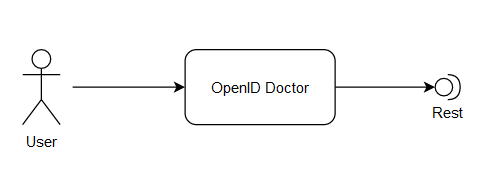
\includegraphics[width=\textwidth]{runtime_comp}
\end{figure}

{\large The OpenID Connect Doctor is standalone CLI tool, should be able to run on as many Operating Systems as possible. }

\newpage
\section{Code Components}
\begin{figure}[!h]
    \centering
    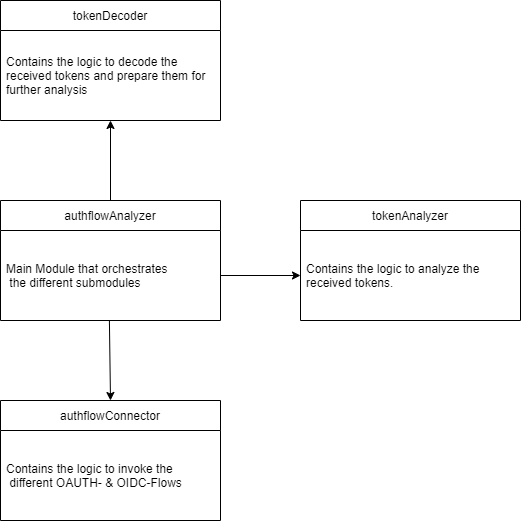
\includegraphics[width=\textwidth]{Code-Components}
\end{figure}


\section{Technology Stack}
\begin{center}
\begin{tabular}{|l|l|l|l|}
    \hline
    \textbf{Tool} & \textbf{Type} & \textbf{Version} & \textbf{Licence} \\\hline
    NodeJS & Programming Language & 16.15.0 & MIT\\
    \hline
    npm & Package Manager & 8.5.5 & MIT\\
    \hline
    Git & Version Control & - & MIT\\
    \hline
\end{tabular}
\end{center}


\end{document}